\chapter{Ordinary Monte Carlo Simulation}
Polish-American mathematician Stanislaw Ulam, recovering from an illness, was playing a lot of
solitary card game. He wanted to calculate the probability of winning and
quickly it is impossible to calculate analytically. Then he thought about playing
lots of hands counting number of wins, but decided it will take years.
After falling several times he asked Von Neumann to build a program to simulate solitary
card game in ENIAC. Then Around 1940 they used Monte Carlo simulation in Manhattan Project
in which physicists wanted to understand how the physical
properties of neutrons would be affected by various possible scenarios following a
collision with a nucleus.

The basis for Monte Carlo is Law of Large Number. If we simulate large number $X_1, X_2, \ldots$ iid
copes of random variable $X$ Then we can approximate the true value $E(f(X))$ by simple mean
$\frac{1}{n}\sum_{i=1}^{n} f(X_i)$. Here in Monte Carlo Random Sampling play the key factor for good estimation of $E(f(X))$.

\section{Evaluate Integrals using Monte Carlo simulation}
The application of Monte Carlo is to computation of integrals. Let $g(x)$ be a function
and suppose we wanted to compute $I$ where
\[
	I = \int_{0}^{1} g(x) dx
\]

To compute the value of $I$, note that if $U\sim U[0,1]$ then we can express $I$ as
\[
	I = E[g(U)]
\]
If $U_1, \ldots, U_n$ are independent uniform $(0,1)$ random variables, it thus follows that
the random variables $g(U_1),\ldots,g(U_n)$ are independent and identically distributed random
variable having mean $I$. Therefore, by law of large numbers, its follows that,
with probability,
\[
	\sum_{i = 0}^{n} \frac{g(U_i)}{n} \to E(g(U))= I \text{ as } k \to \infty
\]

Hence we can approximate $I$ by generating a large number of random numbers $U_i$ and taking
as our approximation the average value of $g(U_i)$.

If we wanted to compute
\[
	I = \int_{a}^{b} g(x) dx
\]
then , by taking the substitute $y=(x-a)/(b-a)$, $dy = dx/(b-a)$, we see that
\begin{align*}
	I & = \int_{0}^{1} g(a+[b-a]y)(b-a)dy \\
	  & = \int_{ 0}^{1} h(y) dy
\end{align*}

Where $h(y)= (b-a)g(a+[b-a]y)$. Thus we can approximate $I$ by continually generating random
numbers and then taking the average value of $h$ evaluated at these random numbers.

Similarly, if we wanted
\[
	I = \int_{0}^{\infty} g(x) dx
\]

we could apply the substitution $y=1/(x+1)$, $dy=-dx/(x+1)^{2} = -y ^{2} dx$, to obtain the identity
\[
	I=\int_{0}^{1} h(y)dy
\]
where, \[
	h(y) = \frac{g(\frac{1}{y} -1)}{y ^{2}}
\]
Using this technique we can also evaluate multidimensional integrals. Suppose that $g$ is a function with n-dimention argument
and we are interested in computing
\[
	I = \int_{0}^{1} \int_{0}^{1} \ldots \int_{0}^{1} g(x_1, x_2 , \ldots , x_n) dx_1 dx_2 \ldots dx_2.
\]
Then, we can express $I$ as
\[
	I = E(g(U_1, U_2, \ldots U_n))
\]
where $U_1, U_2, \ldots U_n \sim U[0,1]$  Hence  if we generate $k$ independent sets, each consisting of $n$ independent $U[0,1]$
random variable
\begin{align*}
	U_1^{1}   & \ldots U_n^{1}  \\
	U_1^{2}   & \ldots U_n^{2}  \\
	          & \vdots          \\
	U_1^{k} , & \ldots, U_n^{k}
\end{align*}
then, since the random variables $g(U_1^{i},\ldots, U_n^{i}), i = 1,2,\ldots,k  $ are all independent and identically distributed
random variable with mean $I$, we can estimate $I$ by $\sum_{i = 1}^{k}g(U_1^{i} , \ldots, U_n^{i} )/k $.

\begin{example}
	Suppose we want to integrate,
	\[
		I = \int_{0}^{1} e^{-\frac{x ^{2}}{2}} dx.
	\]

	Then we can say that,
	\[
		I = E(e^{-\frac{U ^{2}}{2}})
	\]
	where, $U\sim U[0,1]$. Then simulating a large number of $U_1, U_2, \ldots, U_n\sim U[0,1]$ and calculating,
	\[
		\sum_{i = 1}^{n}  \frac{e^{-\frac{U_i ^{2}}{2}}}{n}
	\]
	we can evaluate $I$.

	Hence the algorithm is:\\
	STEP 1: Generate $U\sim U[0,1]$. \\
	STEP 2: Calculate $ e^{-\frac{U ^{2}}{2}} $ and retain it. goto STEP 1. \\
	STEP 3: After large number of iteration evaluate the average.
	\begin{table}[H]
		\begin{center}
			\begin{tabular}{l c}
				\hline
				Monte Carlo sample size & Monte Carlo Estimate of I = 0.8556 \\
				\hline
				50                      & 0.8555                              \\
				100                     & 0.8558                              \\
				1000                    & 0.8555                              \\
				10000                   & 0.8556                              \\
				100000                  & 0.8556                              \\
				\hline
			\end{tabular}
			\caption{Monte Carlo Integration of $e^{-x ^{2}/2}$.}
		\end{center}
	\end{table}
	\begin{figure}[H]
		\centering
		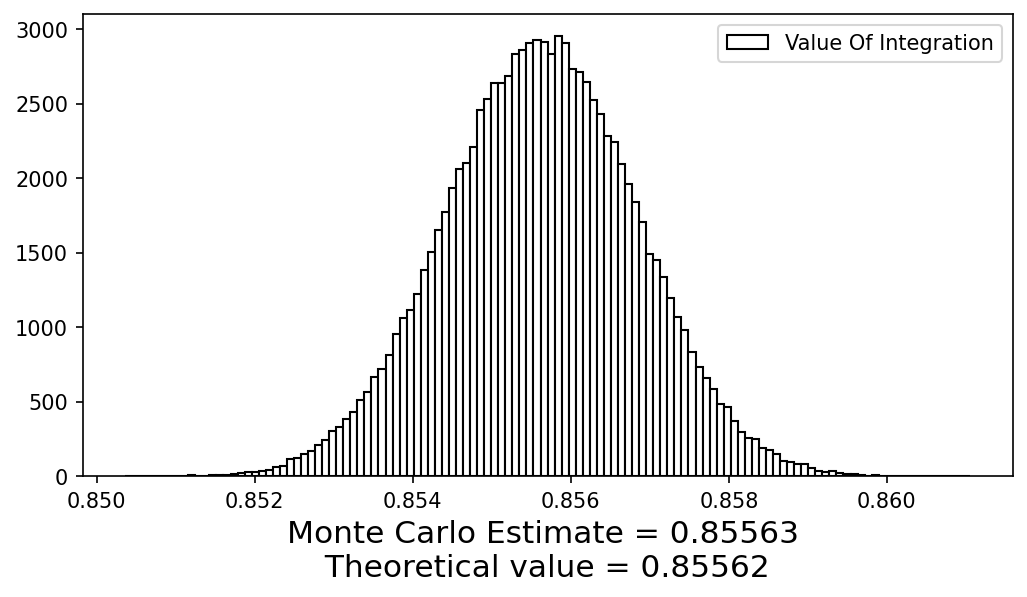
\includegraphics[width=0.6\textwidth]{images/evaluating_integration.png}
		\caption{Monte Carlo Integration of $e^{-x ^{2}/2} $}
	\end{figure}
	Here, we see by the time the Monte Carlo sample size is 100000, we get fairly
	accurate estimates for the value $I$.
\end{example}

\section{The Estimation of $\pi$}
Suppose that the random vector $(X,Y)$ is uniformly distribution in the square of area 4
centered at the origin. That is, it is a random point in the region specified in Figure \ref{Square}.
Let us consider now the probability that this random point in the square in contained within the inscribed circle of radius 1
like the Figure \ref{Circle within Square}.

\begin{figure}[H]
	\centering
	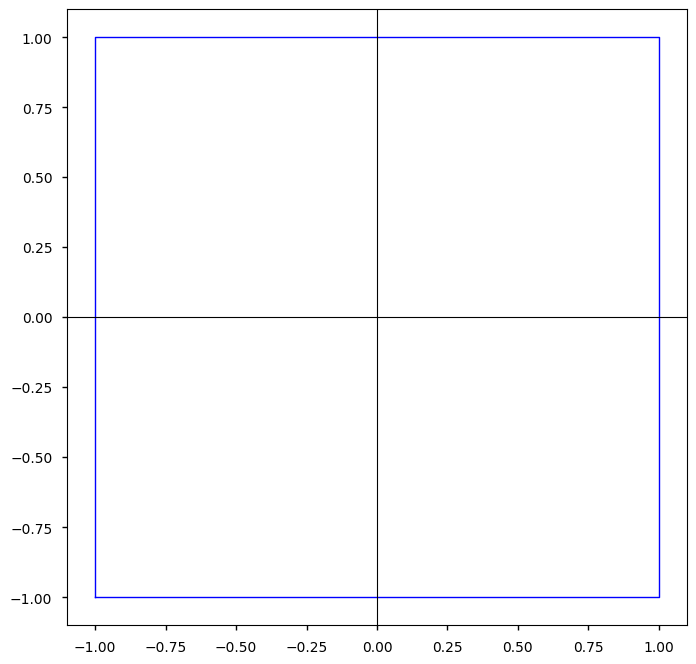
\includegraphics[width=0.4\textwidth]{images/square.png}
	\caption{Square}
	\label{Square}
\end{figure}

\begin{figure}[H]
	\centering
	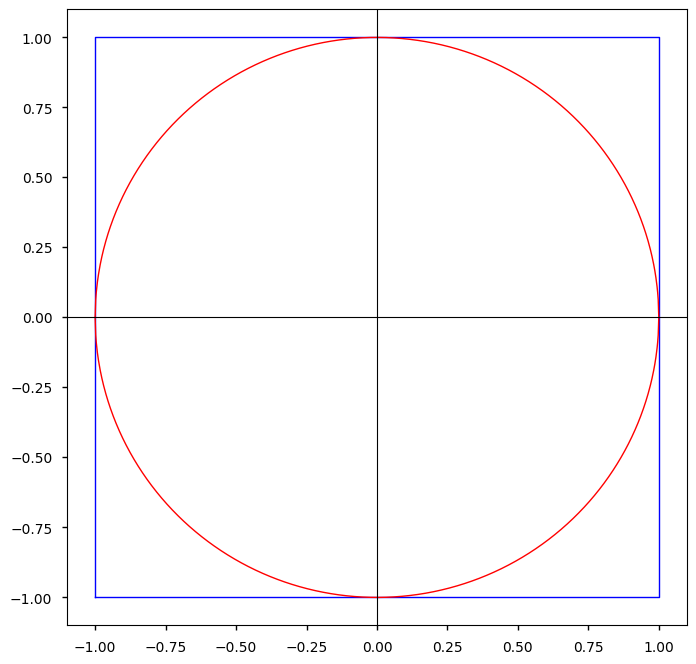
\includegraphics[width=0.5\textwidth]{images/circle.png}
	\caption{Circle within Square}
	\label{Circle within Square}
\end{figure}

Note that since $(X,Y)$ is uniformly distributed in the square it follows that
\begin{align*}
	P((X,Y) \text{ is in the circle } ) & = P(X ^{2}+ Y ^{2}\le 1)                                                        \\
	                                    & = \frac{\text{Area of the circle} }{\text{Area of the square} } = \frac{\pi}{4}
\end{align*}

Hence we generate a large number of points in the square, the proportion of points that fall within the circle will be approximately $\pi/4$.
Now, if $X$ and $Y$ were independent and both were uniformly distributed over $(-1,1)$, their joint density would be
\begin{align*}
	f(x,y) & = f(x)f(y)                                         \\
	       & = \frac{1}{2} \times \frac{1}{2}                   \\
	       & = \frac{1}{4} , \  -1 \le x \le 1,\ -1 \le y \le 1
\end{align*}

Since, the density function of $(X,Y)$ is constant in the square, it thus follows that $(X,Y)$ is uniformly distributed in the square.
Now, if $U\sim U[0,1]$ then $2U\sim U[0,2]$ and so $2U-1\sim U[-1,1]$. Therefore, if we generate ranom numbers $U_1 \text{ and }  U_2$
and set $X=2U_1 - 1$ and $Y= 2U_2-1$, and define,
\[
	I = \begin{cases}
		1 \text{ if } X ^{2} + y ^{2} \le 1 \\
		0 \text{ otherwise }
	\end{cases}
\]
Then,
\[
	E(I)=P(X ^{2} + y ^{2} \le 1) = \frac{\pi}{4}.
\]
Hence the Algorithm for estimating $\pi$ is:\\
STEP 1: Set Circle = 1. \\
STEP 2: Generate $U_1, U_2\sim U[0,1]$\\
STEP 3: If $(2U_1-1)^{2}+ (2U_2-1)^{2} \le 1$ Set Circle = Circle + 1, Otherwise return to STEP 2.
STEP 4: After simulating $N$ time, set $\text{Area of Circle}  = \text{Circle}  / N$

\begin{table}[H]
	\centering
	\begin{tabular}{l c}
		\hline
		Monte Carlo sample & Monte Carlo Estimate of $\pi$ \\
		\hline
		50                 & 2.9600                        \\
		100                & 3.0800                        \\
		1000               & 3.1200                        \\
		10000              & 3.1428                        \\
		100000             & 3.1397                        \\
		1000000            & 3.1394                        \\
		10000000           & 3.1414                        \\
		\hline
	\end{tabular}
	\caption{Monte Carlo Estimates of $\pi$}
	\label{tab:montecarlopi}
\end{table}
Here, we see by the time the Monte Carlo sample size is 10000000, we get fairly accurate estimates for $\pi$


